\section{Integration and extrema without a full grid}
\label{sec:aggregation}
Write $d_s=|\operatorname{dom}P_s|$. There are two different costs of reading a far-away digit. Computing an individual digit at a rational argument may require arithmetic on its address. Enumerating all assignments to every earlier digit can be avoided altogether.

\begin{theorem}[Three constructive observations]\label{thm:agg}
Under (C) and (G) the following rational outputs have error at most $\eps_k$ for the minimum value, the ordinary Riemann integral on $[0,1]$, and the maximum value of the represented function:
\[
       \min_{s\in L_k}v_s,\qquad
       I_k=\sum_{s\in L_k}2^{-d_s}v_s,\qquad
       \max_{s\in L_k}v_s .
\]
All three outputs satisfy the mixed regular-name inequality across levels. A row with maximal value yields a rational point within $2\eps_k$ of the supremum in value. The minimum has the same conclusion.
\end{theorem}
\begin{proof}
Choose $U$ one greater than the greatest address used at level $k$, taking $U=0$ when there are no queries. Among the $2^U$ words of length $U$, exactly $2^{U-d_s}$ extend a prescribed row. Fill each unused address independently to see this bijection, which counts the empty word once at $U=0$. The row families partition the words. Consequently their weights sum to one and $I_k$ is the exact mean of the full table. Repeated reads impose the same constraint and count only once. Any common denominator for the leaf values needs at most another factor $2^{\max_s d_s}$ for this mean, irrespective of $U$.

Given levels $k,l$, use words at their common largest width. For each word the two visited rows are compatible, and (C) bounds their output difference by $\eps_k+\eps_l$. Averaging proves regularity of $I$. Every row at either level has an extension, so the same comparison proves the two extremal inequalities in both directions. This is already an arithmetic derivation of the name contracts. No completed integral or extremum was assumed.

For the integral interpretation, divide $[0,1]$ into the dyadic cells of width $2^{-U}$. At every rational point in a cell interior, the level-$k$ canonical observation is its table entry. The limiting rational-domain value differs from that entry by at most $\eps_k$ by (C). By the proved uniform continuity, this bound extends to the closed cell, including the endpoints (approach from the interior with rational points). Quantitatively, an endpoint can equivalently use that cell's own endpoint expansion, and positive gaps are eliminated by the rational slack argument used for (G). On a dyadic refinement of these cells, each Riemann tag value therefore differs from its parent entry by at most $\eps_k$. The sum of subinterval lengths is one. The tagged sum is within $\eps_k$ of $I_k$. For arbitrary sufficiently fine tagged partitions, refine by their union with the dyadic partition. Compare tags within the original subintervals using the modulus from Theorem~\ref{thm:interval}. Mesh at most $2^{-\mu(j)}$ adds at most $\eps_j$ in total. Thus arbitrary fine rational Riemann sums converge to the name $I$. This proves adequacy with an explicit error estimate and avoids a measure-existence axiom.

For the upper extremum, all rational-domain values are bounded by $\max v_s+\eps_k$, and the bound extends to completed inputs by continuity. Take a maximizing row and set unassigned bits equal to zero. The resulting finite-support expansion gives a rational point with value at least $\max v_s-\eps_k$. The supremum is the named least upper bound. Indeed, all values satisfy the preceding upper estimate, and any proposed upper bound must bound the explicit near-witness at each precision. A rational gap to the name is contradicted by choosing $2\eps_k$ smaller than that gap. Negate outputs to obtain the lower extremum. The near-witnesses need not converge to one maximizing point.
\end{proof}

\begin{figure}[htbp]
\centering
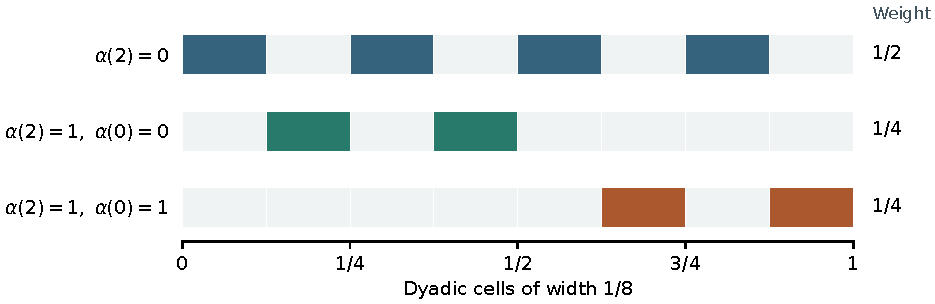
\includegraphics[width=.85\linewidth]{figures/sparse-cylinders.pdf}
\caption{A program first asks for bit 2, and asks for bit 0 only when the reply is one. Color shows the cells reaching each terminal row. The unqueried bit 1 has already been summed out. Row weights require only the number of distinct answers on that path.}
\end{figure}

The averaging proof works on Cantor space already from (C). Condition (G) is what allows us here to speak of an extensional \emph{continuous} function of a Cauchy real. The integral of the first binary digit as a step function also exists, although that digit fails (G). This illustrates the distinction between the finite counting identity and the analytic interface chosen in Theorem~\ref{thm:interval}.

\subsection{A high-frequency calculation}
Let $T(t)=2\min(\{t\},1-\{t\})$, with the periodic extension at integers. For $J\ge0$ consider $f_J(x)=T(2^J x)$. At precision $m\ge1$, read just the $m$ bits with addresses $J,\ldots,J+m-1$. Treat them as the integer $v<2^m$ and return
\[
                   T\big((v+1/2)2^{-m}\big).
\]
On either expansion of any point the fractional phase belongs to the closure of the corresponding phase bin, with $0$ and $1$ identified. Since $T$ is 2-Lipschitz on each period and matches across the boundary, the error is at most $\eps_m$. For level zero use the constant $1/2$. Thus (C) and (G) hold. Each half-period is linear, so the midpoint rule is exact on every bin for $m\ge1$ and the mean is exactly $1/2$. Alternatively, sum the symmetric arithmetic progression of the $2^m$ leaf values. Sparse integration does this computation without representing the $2^J$ periods.
\begin{center}
\begin{tabular}{rrrrr}\toprule
$J$ & sampled digits $m$ & leaves & least exact prefix & mean\\\midrule
0 & 6 & 64 & 6 & $1/2$\\
5 & 6 & 64 & 11 & $1/2$\\
10,000 & 6 & 64 & 10,006 & $1/2$\\\bottomrule
\end{tabular}
\end{center}
For $m=6$, changing the last inspected digit of the first bin changes its midpoint value. The least exact prefix is therefore $J+6$, even though each path reads six bits. A literal prefix table in the last row would have $2^{10006}$ entries. The comparison is with that particular table representation. A specialized formula for the tent's integral also immediately gives $1/2$. The sparse tree works without recognizing that formula.

\subsection{Gluing intervals on a finite metric graph}
Let a finite connected graph have at least one edge, no isolated vertices, and positive rational edge lengths $\lambda_e$. Loop edges and parallel edges are allowed. Give each oriented edge its own unit-interval bit evaluator satisfying (C) and (G). For every two incidences at a vertex require that the two corresponding constant endpoint streams at level $k$ have outputs differing by at most $2\eps_k$, for every $k$. This includes the two ends of a loop. It is a finite scan at fixed $k$. Comparing at an arbitrarily fine intermediate level using (C) proves the mixed endpoint inequalities, hence the edge limits give a common vertex value.

\begin{corollary}[Gluing and averaging on a graph]
These data yield a PR evaluator on regular names for the path metric of the graph, a PR modulus on the whole graph, and a regular name for its normalized arclength integral:
\[
             \frac{\sum_e\lambda_e I_{e,k}}{\sum_e\lambda_e}.
\]
\end{corollary}
\begin{proof}
Take rational edge positions as the dense codes. Distances are rational and PR in the coded finite graph. On one edge include the direct path. Also try each choice of an endpoint of each of the two incident edges, add the initial and terminal partial lengths, and minimize the intervening vertex-to-vertex distance. For the latter enumerate simple vertex paths with their edge choices up to the vertex bound, since removing any cycle shortens a path. The empty path is admitted between identical vertices. This computation proves that a minimum is attained on the finite dense problem.

Let $\mu_e(j+1)$ be the interval modulus already computed at target $j+1$. Choose a dyadic $r=2^{-m}$ with
\[
  0<r\le \tfrac12\min_e\bigl(\lambda_e\,2^{-\mu_e(j+1)}\bigr).
\]
To make this choice by a PR calculation, observe that if the right side is $a/b>0$ for positive integers, $m=b$ works, and bounded minimization up to $b$ gives a smaller exponent if desired. In particular $r$ is strictly shorter than any whole edge. A shortest path of length at most $r$ is therefore direct along an edge, or consists of two partial edges meeting at a single vertex. For either partial segment its normalized length is within the modulus of its edge, so its change in limiting value is at most $\eps_{j+1}$. Equality of the vertex value joins these bounds and gives $\eps_j$ in all cases. At a rational dense point evaluate its chosen edge. The endpoint tests make different incident edge codes equivalent as names. Thus the dense evaluator has a mixed bound with this explicit graph modulus. The Cauchy lift uses the same envelope-and-extra-bits argument as on the interval, now applied to the rational graph distance. In particular one need never choose an edge containing the limit of a Cauchy name. Each normalized edge integral has error $\eps_k$. Taking their convex combination preserves this error and gives the displayed arclength formula by additivity on edges.
\end{proof}
A single loop gives a periodic real domain. The endpoint test detects a simple failure. The identity function on the parameter interval passes the interior carry tests, but its values at the endpoints differ by one and cannot define a continuous function on the loop. For a triangle with edge lengths $1,2,3$ and linearly interpolated cyclic vertex values $0,1,-1$, the three edge means are $1/2,0,-1/2$. The normalized graph integral is therefore $-1/6$. The reference program verifies the three endpoint comparisons at seven precisions.

\subsection{Two limits on automatic modulus extraction}
\paragraph{An evaluation oracle without a clocked program.}
A modulus at tolerance $1/2$ cannot be computed uniformly from pointwise rational evaluations of an otherwise unrestricted continuous function. Run a proposed oracle algorithm on the zero function. It asks for finitely many rational arguments, and returns some $m$. Choose a rational subinterval avoiding all those arguments and shorter than $2^{-m}$. A rational piecewise linear tent supported there with height one agrees on every query but violates the returned modulus. The alternative construction and both evaluators are PR once the finite data are fixed. Hence the clock and transition access used for exploring all possible answers genuinely supply information. A clock for each individual black-box evaluation alone does not expose its branches in the input point.

\paragraph{A computable interval function with no PR modulus.}
Enumerate the unary PR programs effectively, with programs $p_i$. In ordinary computability theory the function $A(n)=1+\max_{i\le n}p_i(n)$ is total computable by interpreting finitely many structurally recursive programs and waiting for their evaluations. It eventually strictly exceeds every unary PR function. Consider
\[
                     g(x)=\sum_{n=1}^\infty 4^{-n}T(2^{A(n)}x).
\]
Its tail after $n$ is bounded by $4^{-n}/3$, and each finite term is computable on Cauchy reals. Computing sufficiently many terms with total error split among them gives a Type-2 computable continuous function in the external interpretation. Yet $g(0)=0$ and at $x_n=2^{-A(n)-1}$ the $n$th summand is $4^{-n}$ while every summand is nonnegative. A modulus at tolerance $2^{-(2n+1)}$ must therefore satisfy $\mu(2n+1)>A(n)+1$. A PR $\mu$ would contradict diagonal domination. The example identifies a specific limitation of embedding Type-2 computable analysis into clocked PR arithmetic even on a compact interval.
